\section{Problem Statement}
\label{sec:introduction:problem-statement}

% Intro problem 
% - Fast growing, but immature
% - Operational & performance challenges
% - - SMI / SMP
% - Non Functional Requirements
% - How to compare systems
% - Balance between performance/reliability

\begin{figure}[!t]
    \centering
    
    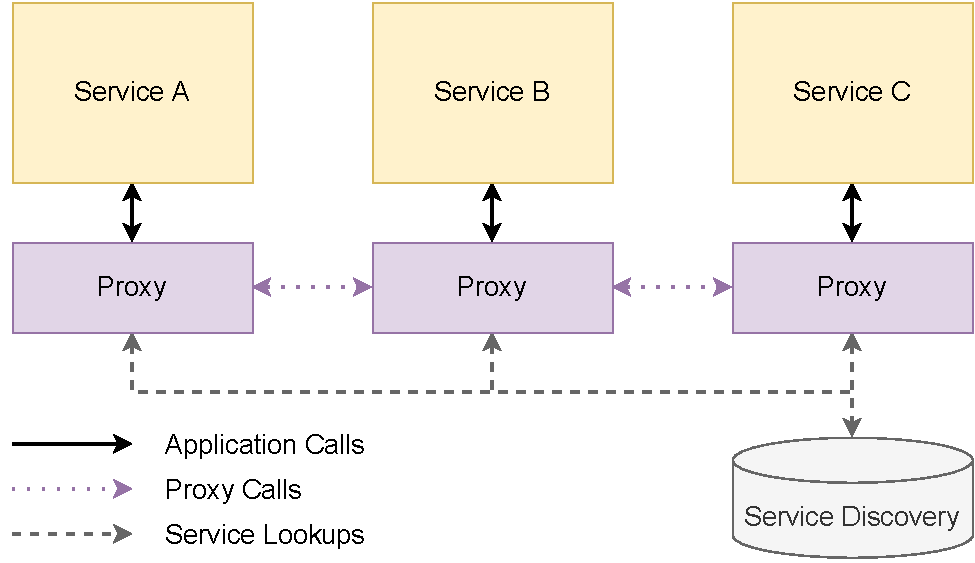
\includegraphics[width=.8\linewidth]{1_introduction/figures/service-mesh-architecture-simple.pdf}

    \caption[Simplistic depiction of a \gls{sm} architecture.]{Simplistic depiction of a \gls{sm} architecture. The core concept is that the service-to-service communications are intercepted and processed by intermediary network proxies.}
    \label{fig:service-mesh-architecture-simplified}
\end{figure}

The \gls{sm} architecture is an emerging approach to address several challenges presented in distributed systems. As a by-product of in the increasingly popular service-oriented design, applications increasingly rely on service-to-service communications over the network. Systems that adhere to a \gls{sm} architecture, aim to abstract away the challenges and intricacies of dealing with unreliable and dynamic networking environments, by introducing a dedicated layer of infrastructure between the applications services. 

The \gls{sm} architecture (see \cref{fig:service-mesh-architecture-simplified}), introduces a set of networking \textit{proxies} to intercept all communications to and from application \textit{services}. These proxies then forward the requests to the original intended recipients whilst dealing with the challenges of a service-oriented design. The proxies are constantly aware of the up-to-date services in a dynamic system, through \textit{service discovery} mechanisms. The proxies establish a uniform layer that can improve the infrastructure in four areas of interest; \textit{observability}, \textit{reliability}, \textit{security} and \textit{programmability} (see background \cref{sec:background:service-mesh}). The outstanding feature of a \gls{sm} architecture is that the underlying services are not aware that their traffic is intercepted. This means that a \gls{sm} system can be introduced without having to modify any application code.

\Gls{sm} systems form a relatively new and exciting field, that is rapidly evolving. However, it is also a field where there is very limited output from the academic world. Specifically, there is very little known about the performance implications of these systems and the additional machinery these systems introduce. The goal of this thesis is to answer this unsolved challenge, and perform an extensive study into performance implications of \gls{sm} systems. 

Before diving into the performance implications of \gls{sm} systems we need to establish an overview of the field by identifying current \gls{sm} systems. After this, we have to figure out what the functional components of a service mesh are and figure out how they differ between the identified systems. During this process, we identify different implementation details and entirely different architectural approaches to the problems they aim to solve. This process allows us to see how the \gls{sm} systems functionally differ from one another. By taking such an approach, we can create a comparison framework, which allows us to objectively compare \gls{sm} systems and allows us to hypothesize on the performance implications.

After we have laid down the groundwork to functionally compare \gls{sm} systems, we have to design and implement a system that can evaluate the performance of them. To properly evaluate \gls{sm} systems and test our hypothesizes, we have to design a benchmark system that captures the performance implications of the functional components of a \gls{sm} system. In this process, we have to clearly define the boundaries of the system and its components that we wish to evaluate. Furthermore, we have to establish a set of metrics that are relevant to \gls{sm} systems and make sure that the benchmark system produces reproducible results. Additionally, we have to create a configurable system that can emulate a wide range of workloads. This allows us to evaluate \gls{sm} systems in various environments.

To thoroughly understand the performance implications of \gls{sm} systems, we have to design a set of experiments that emulate common real-world scenarios. We do this by identifying common workloads in service-oriented architectures. What are the common communication protocols in such environments, and how are they used? By designing experiments that emulate these workloads and using our benchmark system, we can objectively compare the performance implications of \gls{sm} systems. This allows us to perform a quantitative analysis, which enables us to identify performance overheads and potential bottlenecks. Furthermore, it allows us to correlate functional differences and architectural approaches to the quantitive results, enabling an extensive performance analysis. 



% Although there has not been much attention from academia, prior efforts originating from the industry have resulted in a tool \cite{kinvolk-bench} that can capture performance overheads in \gls{sm} systems. This tool lacks in depth and scope, but has laid some groundwork by producing early performance results \cite{bench-istio-linkerd-2019, bench-istio-linkerd-2021}. 


% To fully understand the performance implications of \gls{sm} systems, it is important to know how these systems function under the hood and how they differ from one another. Once we understand these systems in detail, we have to design a benchmark that captures the performance characteristics of \gls{sm} systems. With a benchmark system capable of doing that, we have to design performance oriented experiments that evaluate \gls{sm} systems under various synthetic loads, that emulate common real-world scenarios.



% The \gls{sm} architecture provides modern, distributed systems best practices and tries to solve and minimize the complexities of application developers and system operators alike. It is an area of interest that is actively being worked on in the industry in a rapidly evolving landscape. Although it has gained a lot of interest in the last decade, the technology is in its relative infancy and is facing several challenges from both operational and performance related standpoints. Since it implements a layer of networking abstraction, it creates a potential for a programmable interface, which in turn allows for application and service aware traffic management capabilities. This can differentiate different service mesh implementations based on their capabilities and \glspl{nfr}, where some implementations can support advanced feature sets like circuit breaking behaviour while others do not. Collaborative efforts have are established to create a standard for service meshes \cite{service-mesh-interface, service-mesh-interface-spec}, resulting in the \gls{smi}, a standard interface for service mesh implementations on Kubernetes that describes the most common service mesh capabilities, such as traffic policies, traffic telemetry and traffic management. However, the proposed standard is relatively new, primitive and imposes the question if any existing implementation even accounts for this interface as preliminary research done by us suggests that it does not. Another aspect that is of importance is the performance characteristics of these implementations. How can we characterize the performance characteristics of a \gls{sm} so that we can objectively compare implementations. Through joint efforts, a \gls{cncf} project on a performance specification dubbed \gls{smp} has also been established \cite{service-mesh-performance, service-mesh-interface-spec}. This specification, however, is even newer than the \gls{smi} standard and at the time of writing consists of only the most basic and generic measurements available.

% % Challenges (three chapters/RQ/contributions)
% % - Systems Survey -> Characteristics/SMI spec comparison
% % - Design/Extend perforamnce SMP Spec
% % - Conduct real world experiments
% The goal of this master thesis is to explore the performance characteristics of \gls{sm} implementations using a distributed systems approach. Although, as mentioned, the community has made initial efforts to solve these challenges, the solutions are far from complete nor capture the core elements to fully understand the performance implications of these systems. Also, since both aforementioned collaborative efforts are merely standards and do not carry an official implementation, it can merely act as a guidance in this research. The first challenge is to evaluate existing \gls{sm} implementations according to their characteristics and compare them to their proposed standard. The second challenge is to evaluate the existing performance standard, and if required, design or extend it to capture the core capabilities of a \gls{sm}. Given the many use cases for \gls{sm} systems and the different environments that one such system can run in, it is important to capture all the elements of such a system so that an objective comparison can be made. The final challenge will be to conduct actual experiments that capture these objective results reliably. Given the very dynamic nature of distributed systems, creating such an environment to evaluate this can be a challenge of its own. All of these challenges will guide the research in this thesis in order to evaluate existing \gls{sm} systems.